\documentclass[14pt,a4paper]{extarticle}
\usepackage[T2A]{fontenc}
\usepackage[utf8]{inputenc}
\usepackage[russian]{babel}
\usepackage{geometry}
\usepackage{hyperref}
\usepackage{listings}
\usepackage{graphicx}
\usepackage{float}
\usepackage{xcolor}
\lstset{basicstyle=\ttfamily\small,breaklines=true,frame=single,columns=fullflexible,showstringspaces=false,backgroundcolor=\color{black!3}}
\geometry{left=30mm,right=15mm,top=20mm,bottom=20mm}
\setlength{\parindent}{1.25cm}
\setlength{\parskip}{0.2em}
\sloppy
\begin{document}
\begin{titlepage}
\begin{center}
САНКТ-ПЕТЕРБУРГСКИЙ НАЦИОНАЛЬНЫЙ\\
ИССЛЕДОВАТЕЛЬСКИЙ УНИВЕРСИТЕТ ИТМО
\vspace{1.5cm}

Дисциплина: Бэк-энд разработка
\vspace{1.5cm}

\textbf{Отчет}
\vspace{0.5cm}

Лабораторная работа 5
\vspace{0.5cm}

\textbf{Настройка конфигурации Ansible}
\vfill
\begin{flushright}
Выполнил:\\ Цатинян Артём\\ Группа БР1.2
\vspace{0.8cm}

Проверил:\\ Добряков Д. И.
\end{flushright}
\vfill
Санкт-Петербург\\ 2026 г.
\end{center}
\end{titlepage}
\section{Задача}
Разработать конфигурацию Ansible и плейбук для автоматической настройки виртуальной машины, установки системных пакетов, подготовки окружения и запуска сервисов приложения бронирования столиков из ЛР2.
\section{Ход работы}
\subsection{Архитектура стенда}
Управляющая машина запускает Ansible и подключается к Ubuntu по SSH. На целевой машине устанавливаются Docker, плагин Compose и nginx. Приложение включает сервисы identity, catalog, booking и review, PostgreSQL и RabbitMQ. Nginx направляет запросы с префиксами сервисов на порты 8081--8084.

Управляющая среда --- Ubuntu в WSL на Windows. Виртуальная машина создана в Multipass с Ubuntu 24.04, четырьмя процессорами, 8 ГБ оперативной памяти и диском 30 ГБ. На управляющей машине установлен Ansible Core 2.20.1.
\begin{figure}[H]\centering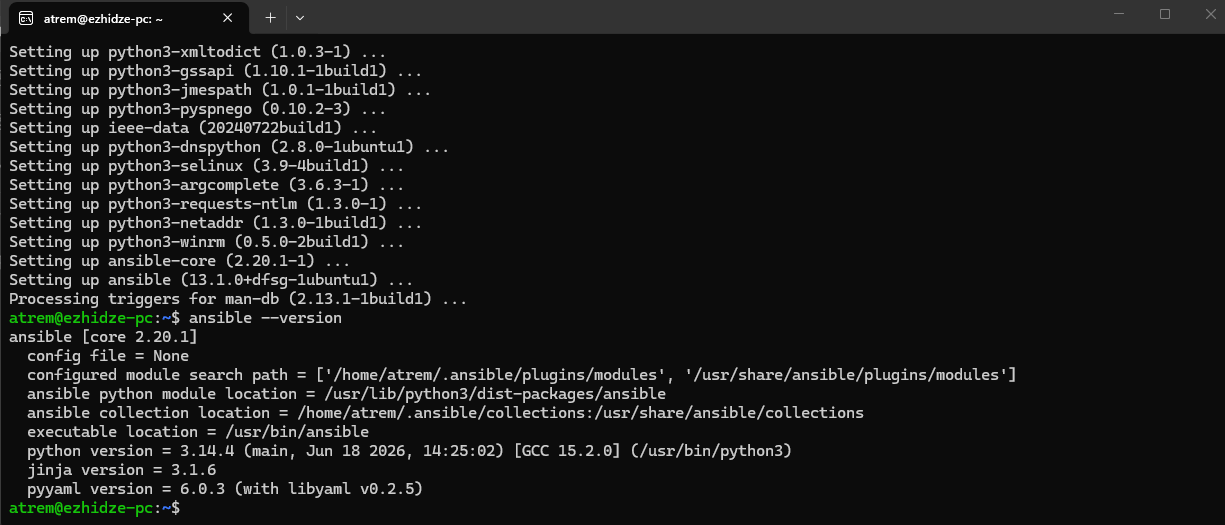
\includegraphics[width=\textwidth]{screenshots/ansible.png}\caption{Установленная версия Ansible}\end{figure}
\begin{figure}[H]\centering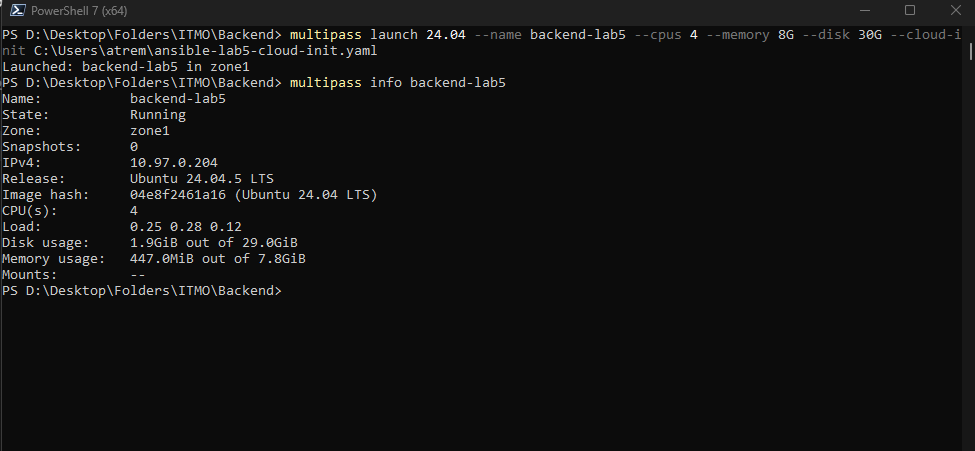
\includegraphics[width=\textwidth]{screenshots/vm.png}\caption{Параметры виртуальной машины Multipass}\end{figure}

Для доступа создан ключ SSH и передан в виртуальную машину через cloud-init. В используемой конфигурации прямое соединение из WSL с адресом ВМ завершалось по тайм-ауту. Для локального подключения применены сетевой режим WSL mirrored и переадресация Windows с адреса 127.0.0.1:2222 на порт 22 виртуальной машины. Проверка выполнена по SSH и модулем Ansible ping.
\begin{figure}[H]\centering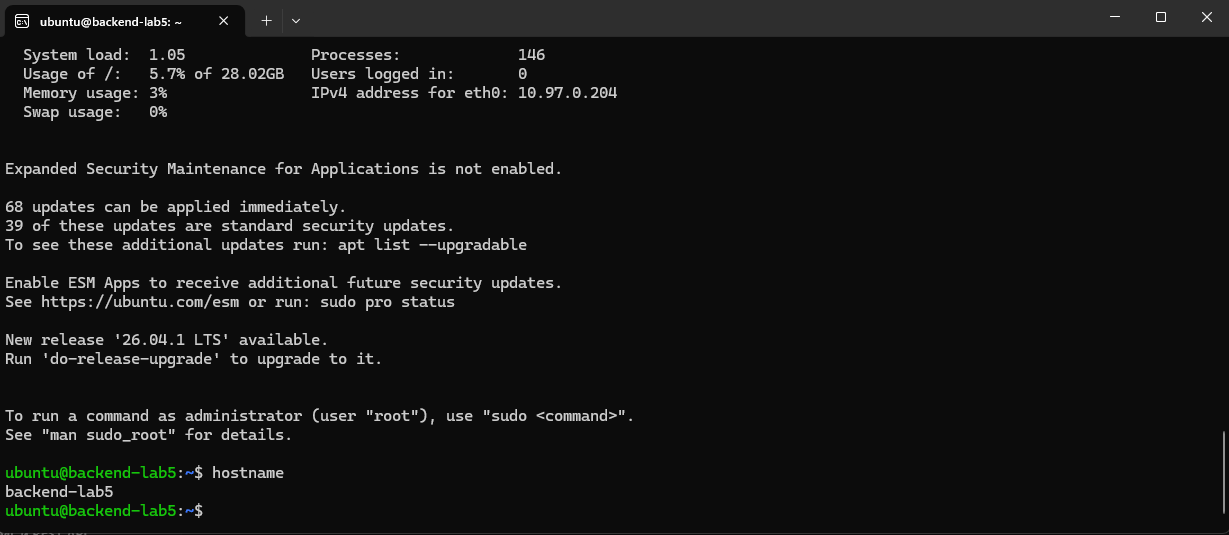
\includegraphics[width=\textwidth]{screenshots/ssh.png}\caption{Подключение к виртуальной машине по SSH}\end{figure}
\begin{figure}[H]\centering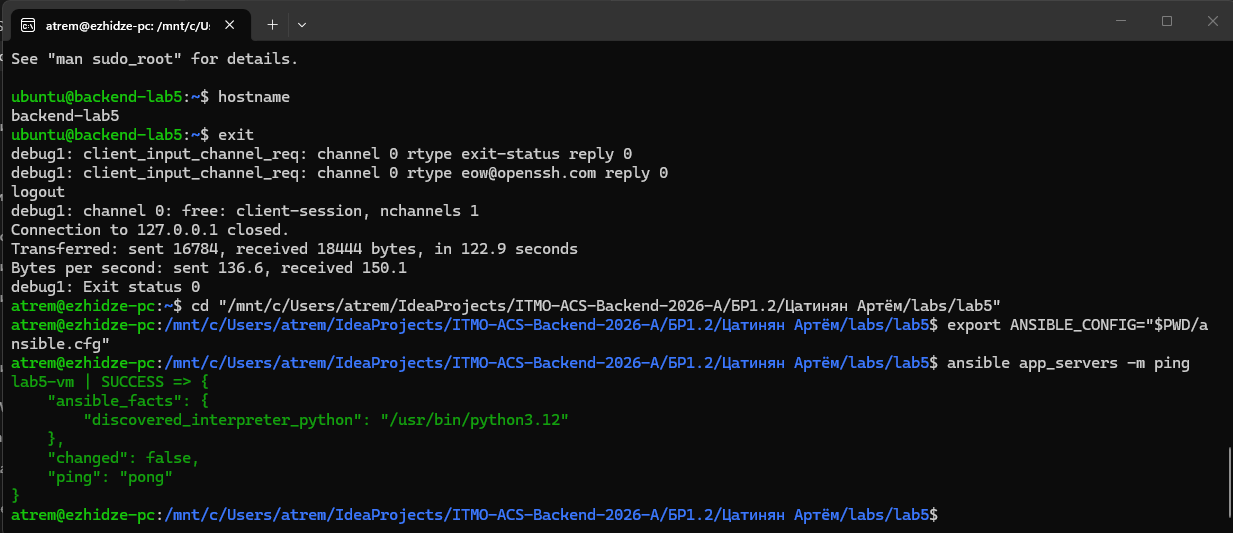
\includegraphics[width=\textwidth]{screenshots/ping.png}\caption{Проверка доступности узла средствами Ansible}\end{figure}
\subsection{Конфигурация и роли}
В inventory описан узел группы app\_servers. Параметры приложения вынесены в group\_vars. Главный плейбук site.yml последовательно применяет роли common, docker, nginx и app. Роль common устанавливает базовые пакеты и часовой пояс; docker устанавливает и запускает Docker; nginx устанавливает прокси из шаблона и применяет конфигурацию через обработчики. Роль app копирует исходники ЛР2 и запускает Docker Compose со сборкой образов. Кэш и сборочные каталоги исключены из копирования.

Конфигурация размещена в каталоге labs/lab5. Файл ansible.cfg задаёт путь к inventory и ролям, inventory.ini содержит параметры SSH-подключения, а group\_vars/app\_servers.yml --- путь установки и список сервисов с портами. В каталоге roles находятся задачи и шаблон конфигурации nginx. Главный плейбук применяет четыре роли к группе серверов:
\begin{lstlisting}
hosts: app_servers
become: true
roles:
  - common
  - docker
  - nginx
  - app
\end{lstlisting}

Повышение привилегий become необходимо для установки системных пакетов, управления службами и записи файлов в /opt и /etc/nginx. Роль common устанавливает curl, git, rsync, Python и сертификаты, после чего задаёт часовой пояс Europe/Moscow. Роль docker устанавливает пакеты docker.io и docker-compose-v2 и включает системную службу Docker.

Роль nginx создаёт конфигурацию из шаблона Jinja2 и включает сайт. Для каждого сервиса в шаблоне формируется отдельное расположение с проксированием на соответствующий локальный порт. При изменении конфигурации обработчики сначала выполняют проверку nginx -t, затем перезагружают службу; до начала итоговых проверок изменения применяются с помощью flush\_handlers.

Роль app создаёт каталог /opt/restaurant-booking, копирует исходники через synchronize и исключает локальные сборочные каталоги и журналы. Затем запускается команда docker compose up -d --build. Для подключения приложений к PostgreSQL и RabbitMQ используется сеть Compose; параметры межсервисных URL передаются контейнерам в переменных окружения.

Пути /identity/, /catalog/, /booking/ и /review/ проксируются на соответствующие сервисы. После запуска плейбук ожидает ответ HTTP 200 от OpenAPI каждого сервиса через nginx. Это подтверждает доступность HTTP-интерфейсов, но не заменяет проверку всех бизнес-сценариев.

Для загрузки образов на стенд используется зеркало mirror.gcr.io: при обращении к первоначальному реестру загрузка слоёв завершалась по тайм-ауту. Плейбук формирует копии Compose и Dockerfile с адресами зеркала, сохраняя исходные файлы ЛР2. При копировании скрипта Gradle дополнительно устраняются окончания строк CRLF, несовместимые с запуском через Linux shebang.

\subsection{Возникшие трудности}
При настройке стенда прямое SSH-соединение между WSL и виртуальной машиной не устанавливалось. Доступ обеспечен локальной переадресацией порта Windows. При загрузке образов из первоначального реестра возникал тайм-аут; проверка показала, что образ PostgreSQL доступен из альтернативного реестра. После изменения адресов образов сборка продолжилась.

Следующая ошибка возникла из-за окончаний строк в gradlew: Windows-версия файла содержала последовательность CRLF, поэтому Linux не находил интерпретатор скрипта. Проверка первых байтов файла подтвердила наличие символа CR; добавленная в роль задача преобразует окончания строк на целевой ВМ. При первом старте приложения сервисы отвечали не сразу, поэтому итоговая проверка выполняется с повторными попытками.
\subsection{Проверка}
Перед запуском проверены синтаксис и список задач. Плейбук выполнен повторно после устранения проблем с доступом к реестру и окончаниями строк. В итоговом запуске проверки четырёх сервисов завершились успешно: PLAY RECAP показал ok=17, changed=4, unreachable=0 и failed=0. Сначала при запуске сервисов потребовались повторные запросы до готовности identity-service.
\begin{figure}[H]\centering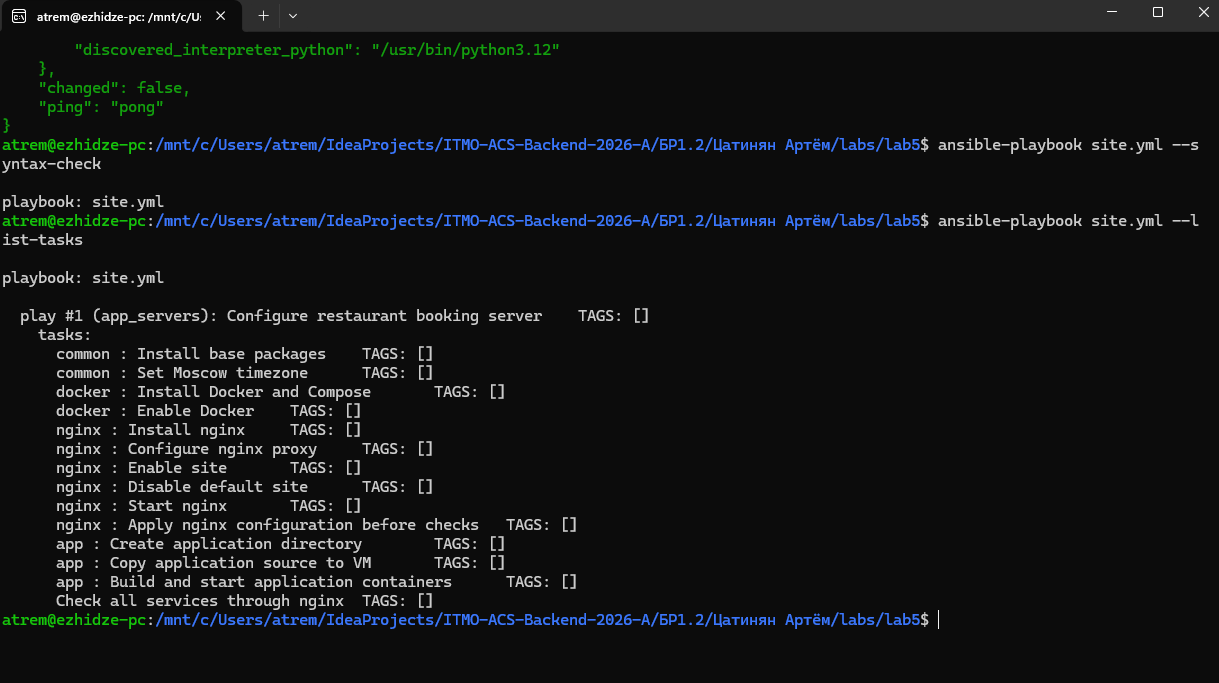
\includegraphics[width=\textwidth]{screenshots/tasks.png}\caption{Проверка синтаксиса и перечня задач}\end{figure}
\begin{figure}[H]\centering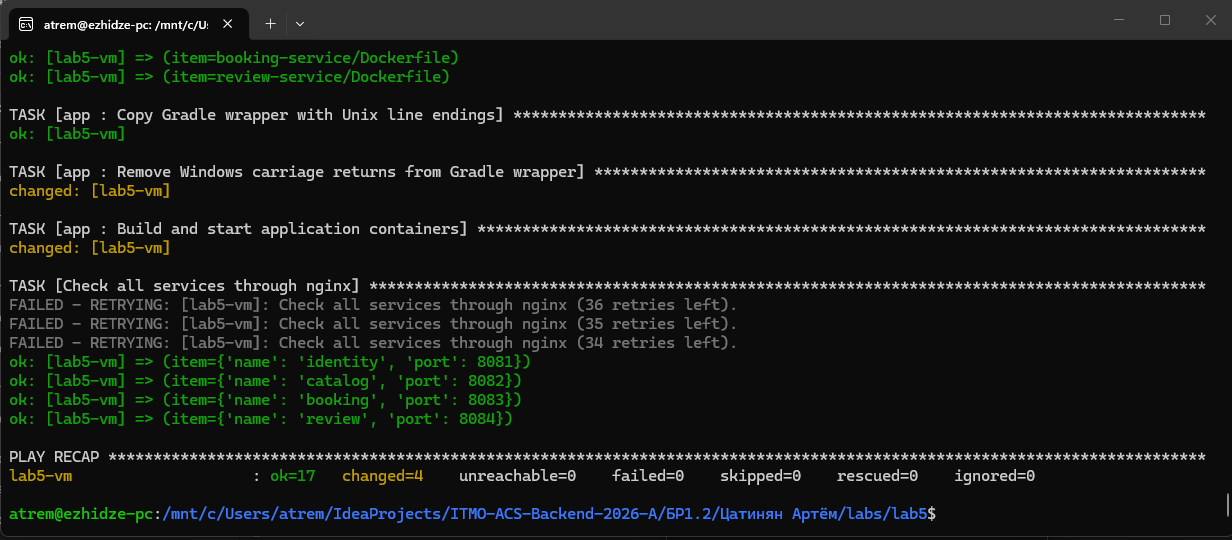
\includegraphics[width=\textwidth]{screenshots/recap.png}\caption{Результат выполнения плейбука и проверок API}\end{figure}

Команда docker ps показала четыре работающих контейнера приложения и два инфраструктурных контейнера. Для PostgreSQL и RabbitMQ отображён статус healthy. Команда Compose выполняется при повторном запуске; в текущей реализации присутствуют изменения, поэтому строгая идемпотентность всего процесса не подтверждена.
\begin{figure}[H]\centering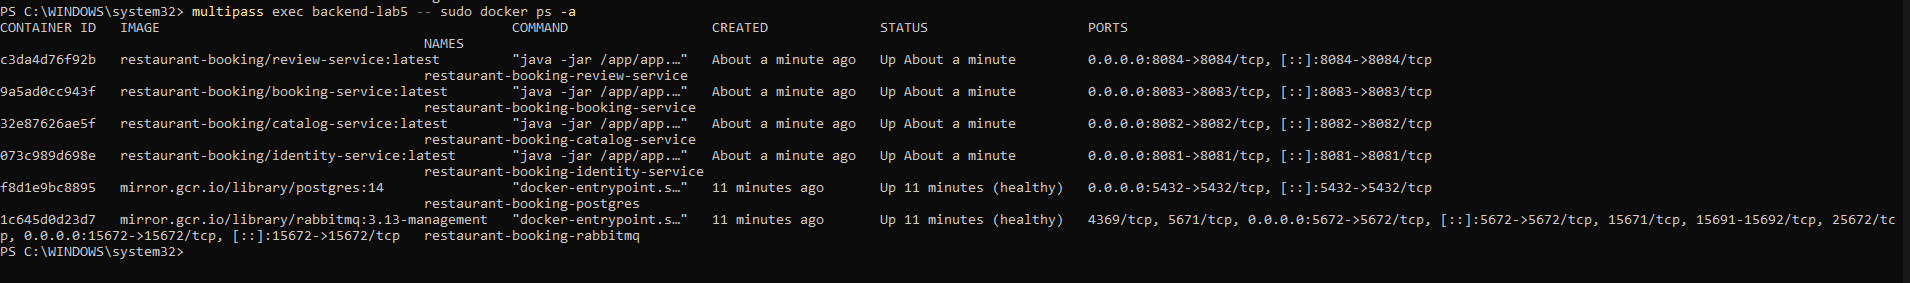
\includegraphics[width=\textwidth]{screenshots/containers.png}\caption{Состояние контейнеров приложения и инфраструктуры}\end{figure}
\subsection{Подготовка системных ресурсов и межсетевого экрана}
Роль common дополнена настройкой файла подкачки /swapfile-lab5 размером 2 ГиБ. При отсутствии файла роль выделяет место, устанавливает права 0600 и выполняет mkswap. После проверки активных устройств файл подключается командой swapon, а запись в /etc/fstab обеспечивает его подключение после перезагрузки. Существующий файл повторно не форматируется.

Для фильтрации входящих соединений установлен и включён UFW. В правила добавлены SSH на порту 22 и HTTP на порту 80; для остальных входящих подключений к хосту задана политика deny. Опубликованные Docker порты могут обрабатываться отдельными правилами перенаправления, поэтому один вывод ufw status не подтверждает их недоступность извне.

\subsection{Проверка на чистой виртуальной машине}
Для дополнительной проверки создана отдельная виртуальная машина backend-lab5-clean с Ubuntu 24.04, четырьмя процессорами, 8 ГиБ оперативной памяти и диском 30 ГБ. Открытый SSH-ключ передан при создании через cloud-init. Подключение управляющей среды к новому узлу проверено модулем Ansible ping, после чего проверены синтаксис плейбука и его выполнение.
\begin{figure}[H]\centering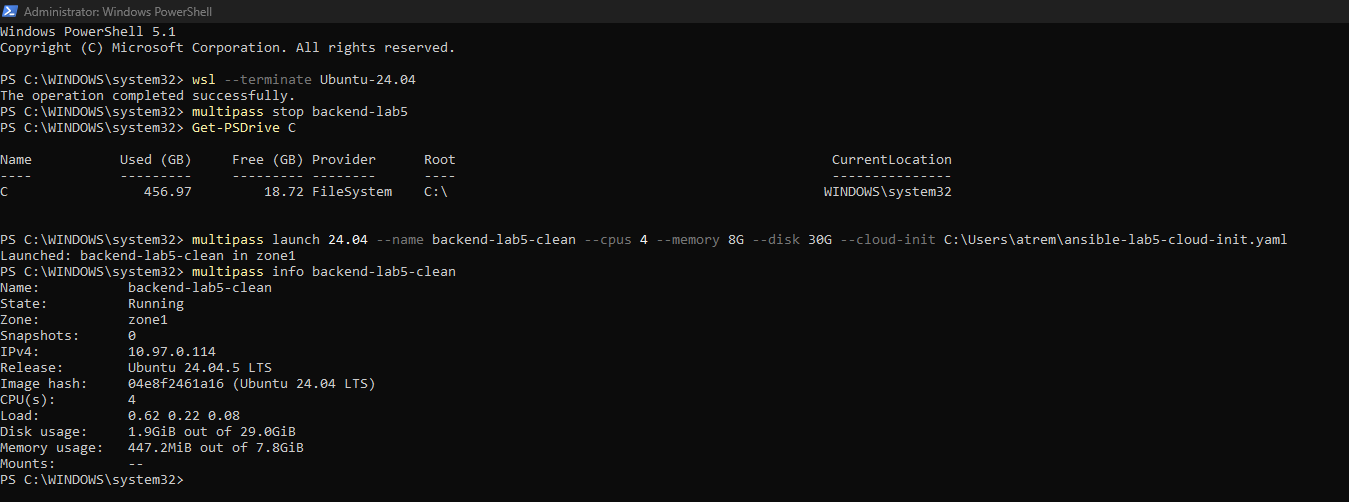
\includegraphics[width=\textwidth]{screenshots/clean-vm.png}\caption{Создание отдельной виртуальной машины для проверки}\end{figure}
\begin{figure}[H]\centering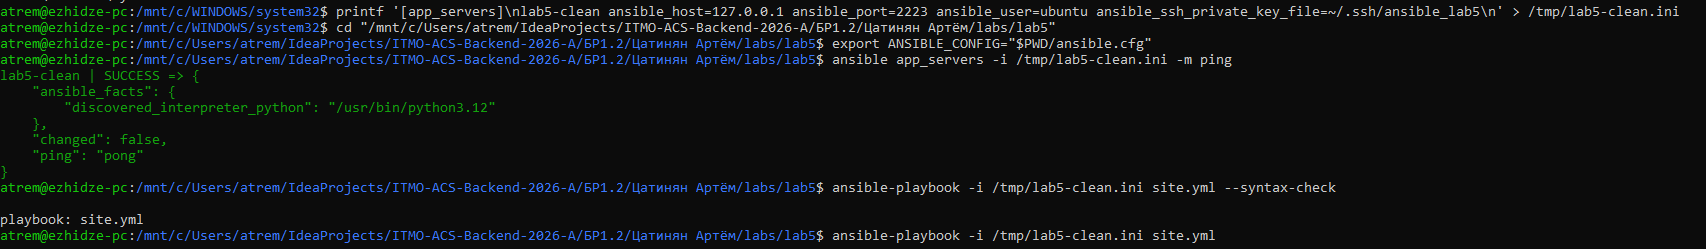
\includegraphics[width=\textwidth]{screenshots/clean-ping.png}\caption{Проверка SSH-соединения и синтаксиса плейбука}\end{figure}

На новом узле первый запуск выявил ошибку команды проверки активной подкачки; параметры swapon исправлены. После прерванной сборки плейбук был запущен повторно и завершился с результатом ok=23, changed=1, unreachable=0, failed=0. Проверки через nginx подтвердили доступность всех четырёх сервисов. Сообщения RETRYING при старте означают ожидание готовности и завершились успешными проверками.
\begin{figure}[H]\centering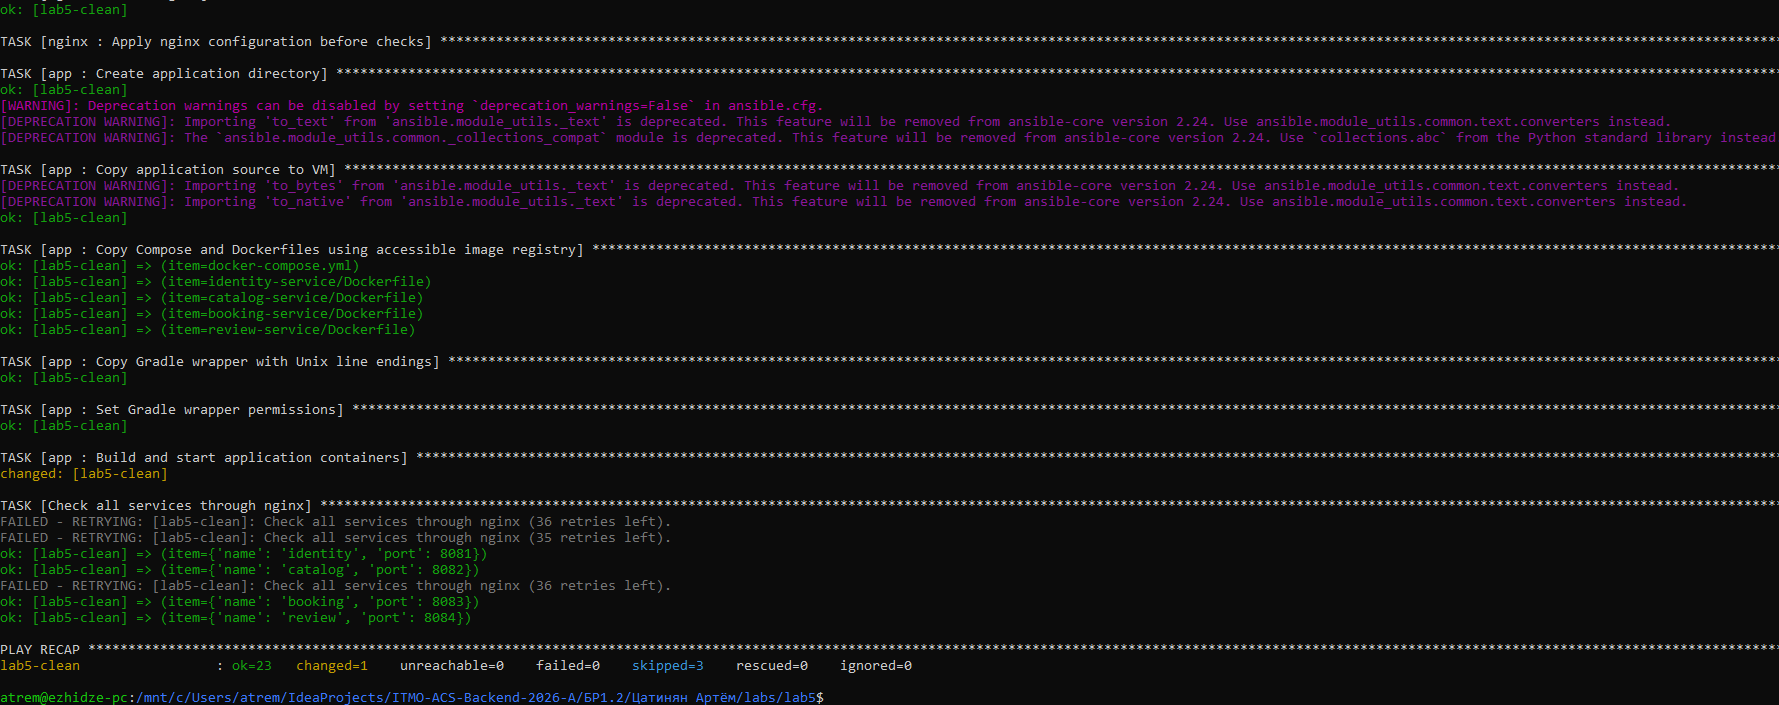
\includegraphics[width=\textwidth]{screenshots/clean-recap.png}\caption{Результат развёртывания на отдельной виртуальной машине}\end{figure}

Дополнительно команда free показала 2 ГиБ подкачки, ufw status --- активные правила для SSH и HTTP, а docker ps --- четыре запущенных сервиса приложения и два инфраструктурных контейнера. Для PostgreSQL и RabbitMQ отображается healthy.
\begin{figure}[H]\centering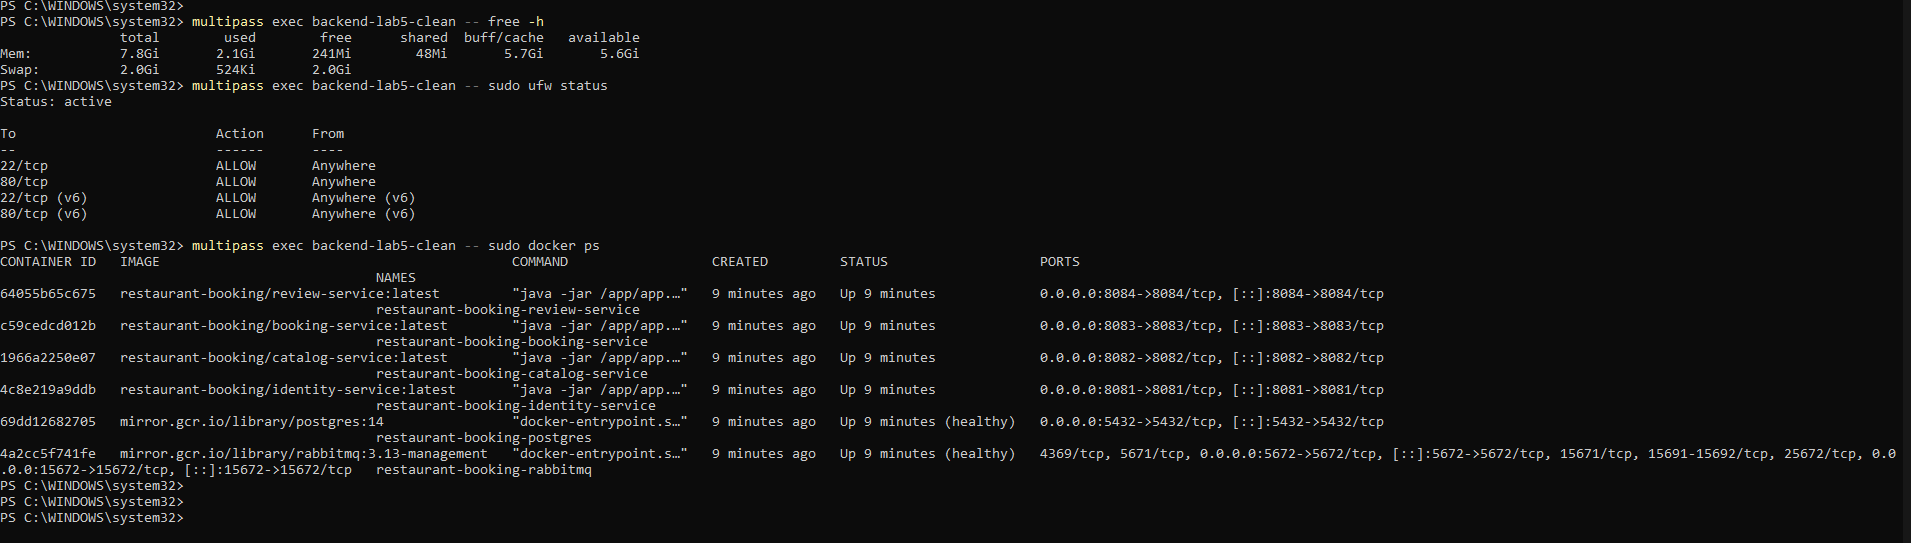
\includegraphics[width=\textwidth]{screenshots/clean-system.png}\caption{Подкачка, правила UFW и контейнеры на проверочной машине}\end{figure}

Для диагностики сборки предусмотрена запись вывода Docker Compose в /var/log/lab5-compose.log. При повторном применении плейбука синхронизация файлов выполняется с проверкой содержимого; полная идемпотентность сборки и запуска контейнеров требует отдельной проверки повторного выполнения.
\section{Вывод}
Разработана и проверена конфигурация автоматической настройки Ubuntu и запуска микросервисного приложения. Ansible установил необходимые пакеты, настроил подкачку, UFW, nginx и Docker, развернул контейнеры и проверил доступность четырёх сервисов через прокси. Работоспособность подтверждена на отдельной виртуальной машине.
\end{document}
